%%% LaTeX Template
%%% This template can be used for both articles and reports.
%%%
%%% Copyright: http://www.howtotex.com/
%%% Date: February 2011

%%% Preamble
\documentclass[paper=a4, fontsize=11pt]{scrartcl}	% Article class of KOMA-script with 11pt font and a4 format
\usepackage[margin=0.7in]{geometry}
\usepackage[english]{babel}															% English language/hyphenation
\usepackage[protrusion=true,expansion=true]{microtype}				% Better typography
\usepackage{amsmath,amsfonts,amsthm}										% Math packages
\usepackage[pdftex]{graphicx}														% Enable pdflatex
%\usepackage{color,transparent}													% If you use color and/or transparency
\usepackage[hang, small,labelfont=bf,up,textfont=it,up]{caption}	% Custom captions under/above floats
\usepackage{epstopdf}																	% Converts .eps to .pdf
\usepackage{subfig}																		% Subfigures
\usepackage{booktabs}																	% Nicer tables


%%% Advanced verbatim environment
\usepackage{verbatim}
\usepackage{fancyvrb}
\DefineShortVerb{\|}								% delimiter to display inline verbatim text


%%% Custom sectioning (sectsty package)
\usepackage{sectsty}								% Custom sectioning (see below)
\allsectionsfont{%									% Change font of al section commands
	\usefont{OT1}{bch}{b}{n}%					% bch-b-n: CharterBT-Bold font
%	\hspace{15pt}%									% Uncomment for indentation
	}

\sectionfont{%										% Change font of \section command
	\usefont{OT1}{bch}{b}{n}%					% bch-b-n: CharterBT-Bold font
	\sectionrule{0pt}{0pt}{-5pt}{0.8pt}%	% Horizontal rule below section
	}


%%% Custom headers/footers (fancyhdr package)
\usepackage{fancyhdr}
\pagestyle{fancyplain}
\fancyhead{}														% No page header
\fancyfoot[C]{\thepage}										% Pagenumbering at center of footer
\renewcommand{\headrulewidth}{0pt}				% Remove header underlines
\renewcommand{\footrulewidth}{0pt}				% Remove footer underlines
\setlength{\headheight}{13.6pt}

%%% Equation and float numbering
\numberwithin{equation}{section}															% Equationnumbering: section.eq#
\numberwithin{figure}{section}																% Figurenumbering: section.fig#
\numberwithin{table}{section}

\usepackage[parfill]{parskip}
\usepackage{float}
\usepackage{graphicx}
\usepackage{hyperref}
\usepackage[numbers]{natbib}															% Tablenumbering: section.tab#


%%% Title	
\title{ \vspace{-1in} 	\usefont{OT1}{bch}{b}{n}
		\huge \strut Development of Vesuvio Data Reduction and Analysis in Mantid \strut \\
}
\author{ 									\usefont{OT1}{bch}{m}{n}
        Samuel Jackson\\		\usefont{OT1}{bch}{m}{n}
        ISIS Facility\\	\usefont{OT1}{bch}{m}{n}
        Rutherford Appleton Laboratory\\
        \texttt{samuel.jackson@stfc.ac.uk}
}
\date{\today}

%%% Begin document
\begin{document}
\maketitle
\clearpage
\tableofcontents
\clearpage
\section{Introduction}
\label{sec:introduction}
VESUVIO is an neutron spectrometer at the ISIS pulsed neutron source operating a high energy range of between 5-150 eV and uses the experimental technique known as neutron Compton scattering to measure the momentum distributions of condensed matter systems \citep{mayers2012vesuvio}. It is located on the S2 beamline and features 64 forward scattering Yttrium Aluminium Perovskite (YAP) gamma ray detectors and 132 $^{6}$Li doped neutron detectors \citep{mayers2011calibration}.

Mantid \citep{mantid} is a data analysis application for neutron and muon scattering data used by multiple facilities across the world. Recently, extensive work has been carried out to integrate the bespoke data reduction and analysis routines with the Mantid framework. While the programs described in this document are designed to replicate the functionality of the Fortran and Genie routines already in use, most of them have been written from scratch and are not based on the original code base. This document outlines the current progress of development regarding what has already been implemented and what is remains to be finished.

\section{Loading}
\label{sec:loading}
In the original data analysis package used two separate commands to process the raw time-of-flight data, one for the front scattering detectors and one for the back scattering. In the Mantid implementation this has been replaced with a single algorithm called LoadVesuvio which performs all of the processing for raw files from the instrument. This includes options for handling each of the different foil positions and difference techniques available with VESUVIO \citep{schooneveld2006foil, mayers2004vesuvio} and summing multiple runs. It also contains a flag for summing each spectrum in the desired range into a single spectrum. The results of this loading operation are output as a single workspace in Mantid with units in time-of-flight.

\begin{figure}[H]
\centering
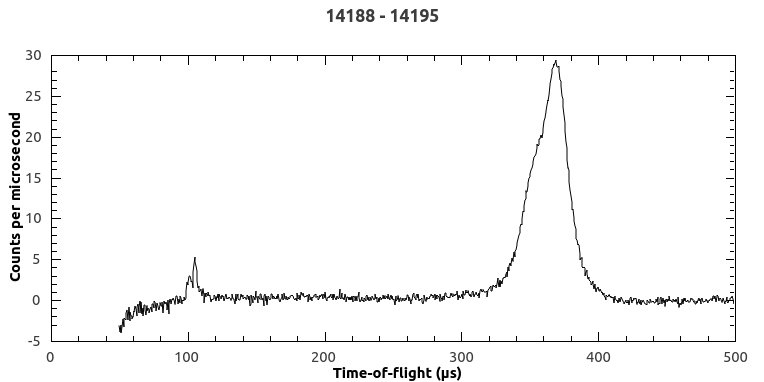
\includegraphics[width=0.6\textwidth]{img/tof-spectrum.png}
\caption{Plot of time-of-flight data from the sum runs 14188-14195 and the sum of detectors 40-134.}
\label{fig:tof-spectrum}
\end{figure}

Optionally, an instrument parameter file can be supplied to the loading routine. This file contains a set of calibrated instrument parameters for each of the detectors and can correct each of the default parameters used and attach $t0$ (the time delay offset parameter) to the instrument attached to the workspace. 

\section{Corrections}
\label{sec:corrections}
The time-of-flight data loaded using the methods described in section \ref{sec:loading} need to be corrected to account for the effects of multiple scattering \citep{mayers2002multiple} and gamma background \citep{mayers2011calculation}. Currently, the multiple scattering corrections for VESUVIO in Mantid have not yet been completed. Corrections for the gamma background are implemented using the Mantid algorithm framework as an algorithm called CalculateGammaBackground. This takes a single workspace in time-of-flight, a fit function describing the mass spectrum of the input data and a list of workspace indices to include as part of the correction. The fit function for the mass spectrum is typically one which has been created as part of the fit routines described in section \ref{sec:fitting}. This algorithm results in two workspaces: one that contains the calculated background and a copy of the input time-of-flight workspace with the background subtracted.

\begin{figure}[H]
\centering
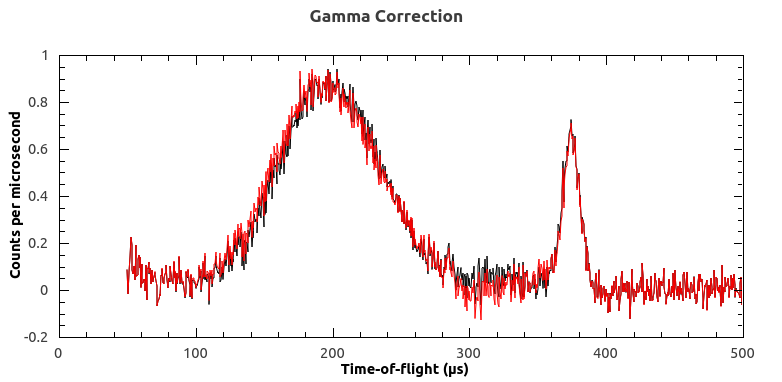
\includegraphics[width=0.6\textwidth]{img/corrections-gamma.png}
\caption{Plot of a Zirconium Hydride (ZrH$_2$) sample. Back is the uncorrected sample, red shows the same sample after gamma correction.}
\label{fig:corrections-gamma}
\end{figure}

\section{Fitting}
\label{sec:fitting}
The majority of the development for integrating VESUVIO into Mantid has concerned the development of the fitting procedures required to measure the neutron compton profile following the theory described in Refs.\citep{mayers2012vesuvio}. Development in this area has focussed on two major additions to the Mantid framework. First was the creation a new suite of fit functions was required which could accurately describe the results of a neutron Compton scattering experiment. The second was the creation of a collection of supporting data analysis routines which setup a fit given the appropriate parameters or the sample. 

The first part has been fully implemented as a collection of new Mantid fit functions, while the second has been created as a separate python package which can be used alongside Mantid. When the design of the data analysis routines is finalised the python analysis package will most likely be better integrated with the Mantid algorithm framework.

\begin{figure}[H]
\centering
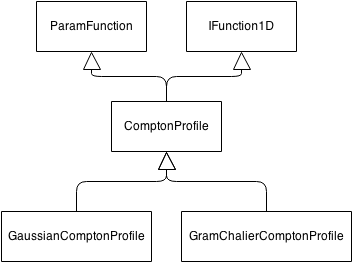
\includegraphics[width=0.4\textwidth]{img/uml/compton-class-diagram.png}
\caption{Class diagram of the Compton Profile fit functions in Mantid.}
\label{fig:compton-class-diagram}
\end{figure}

There are two major fit functions used in the analysis of VESUVIO data. The GaussianComptonProfile defines a function for fitting the simpler Gaussian approximation to mass peaks. The GramChalierComptonProfile is for the more complex fitting case where the atoms in the sample are affected by anisotropy and anharmonicity. Both of these are described in detail in Refs. \citep{mayers2012vesuvio}.

Both of these fit functions inherit from a common class called the ComptonProfile. This implements the common operations between both fit functions such as conversion of time-of-flight data to y-space and the calculation of the resolution components.


\section{Diffraction}
\label{sec:diffraction}
Diffraction on VESUVIO is not yet fully implemented within Mantid. As the reduction of diffraction data is fairly trivial in comparison to the other requirements of VESUVIO data analysis, this can be handled by the existing IndirectDiffractionReduction routine that is used as part of the 

\section{Calibration}
\label{sec:calibration}

\section{GUI}
\label{sec:GUI}

\section{Visualisation}
\label{sec:visualisation}


\bibliographystyle{unsrtnat_corrected}
\bibliography{references}
\end{document}